% -*- TeX:de -*-
\NeedsTeXFormat{LaTeX2e}
\documentclass[12pt,a4paper]{article}
\usepackage[english]{babel} % german text
\usepackage[DIV12]{typearea} % size of printable area
\usepackage[T1]{fontenc} % font encoding
%\usepackage[latin1]{inputenc} % most likely on Windows
\usepackage[utf8]{inputenc} % probably on Linux
\usepackage{multicol}
% PLOTTING
\usepackage{pgfplots}
\usepackage{pgfplotstable}
\usepackage{url}
\usepackage{graphicx} % to include images
\usepackage{tikz}
\usepackage{subfigure} % for creating subfigures
\usepackage{amsmath} % a bunch of symbols
\usepackage{amssymb} % even more symbols
\usepackage{booktabs} % pretty tables
\usepackage{makecell} % multi row table heading
% a floating environment for circuits
\usepackage{float}
\usepackage{caption}
\usepackage{hyperref}
\usepackage{eurosym}

% Title Page command
\newcommand{\HRule}{\rule{\linewidth}{0.5mm}}

%\newfloat{circuit}{tbph}{circuits}
%\floatname{circuit}{Schaltplan}
% a floating environment for diagrams
%\newfloat{diagram}{tbph}{diagrams}
%\floatname{diagram}{Diagramm}
\pgfplotsset{compat=1.8}
\selectlanguage{english} % use german
\begin{document}
%%%%%%% DECKBLATT %%%%%%%
\begin{titlepage}
\begin{center}

% Upper part of the page. The '~' is needed because \\
% only works if a paragraph has started.

\includegraphics[scale=0.75]{./unilogo}~\\[2cm]

\textsc{\LARGE University of Vienna }\\[0.5cm]
\textsc{\LARGE Faculty of Physics}\\[1.5cm]
\textsc{\Large Quantum optics practical course}\\[0.5cm]

% Title
\HRule \\[0.4cm]
{ \huge \bfseries Radiaton Pressure}\\[0.4cm]

\HRule \\[1.5cm]

% Author and supervisor
\begin{minipage}{0.4\textwidth}
\begin{flushleft} \large
\emph{Author:}\\
Johannes \textsc{Kurz}\\
\emph{Group:}\\
\textsc{Braun, Donabaum, Kurz}\\
\end{flushleft}
\end{minipage}
\begin{minipage}{0.4\textwidth}
\begin{flushright} \large
\emph{Supervisor:} \\
Witlef \textsc{Wieczorek}
\end{flushright}
\end{minipage}

\vfill

% Bottom of the page
{\large 31.10.2014}

\end{center}
\end{titlepage}
%%%%%%% DECKBLATT ENDE %%%%%%%
\pagebreak
\setlength{\columnsep}{20pt}

\begin{abstract}
\noindent
In this work we demonstrate that light creates pressure. On a oscillator with a length of 1mm we could show a physical displacement of about 10nm which is significant enough to be caused by the radiation other then side effects (like thermal movement). Also this shows that a cheap table top experiment is sufficient to show this effect.
\end{abstract}

%%%%%%%%%%%%%%%%%%%%%%%%%%%%%%%%%%%%%%%%%%%%%%%%
%\begin{figure}[H]
% \centering
% \includegraphics[scale=0.35]{./data/beugung.png}
% \caption{Beugungsmuster Einzelspalt (echtes Foto; schwarz durch weiß ersetzt)}
% \label{fig:beugungsmuster}
%\end{figure}
%\begin{figure}[H]
% \centering
% \pgfplotstabletypeset[
% columns={abstand, n},
% col sep=&,
% columns/abstand/.style={precision=2, zerofill, column name=\makecell{$Abstand$\\$(\pm 0.05)[mm]$} },
% columns/n/.style={column name=\makecell{$n$\\$(Ordnung)$}, precision=0},
% every head row/.style={before row=\hline,after row=\hline\hline},
% every last row/.style={after row=\hline},
% every first column/.style={column type/.add={|}{} },
% every last column/.style={column type/.add={}{|} }
% ]{
% abstand & n
% 12.9 & 1
% 24.45 & 2
% 37.40 & 3
% 49.35& 4
% 62.45 & 5
% 74.45 & 6
% 87.45 & 7
% 100.25 & 8
%
% }
% \caption{Messwerte Einzelspalt}
% \label{tab:werte_einzelspalt}
%\end{figure}
%%%%%%%%%%%%%%%%%%%%%%%%%%%%%%%%%%%%%%%%%%%%%%%%
%%%%%%%%%%%%%%%%%%%%%%%%%%%%%%%%%%%%%%%%%%%%%%%%


\section{Introduction}
Goal of this work is to demonstrate how photons create pressure on a cantilever which acts as a mechanical harmonic oscillator.\\
On the following pages the theoretical basics will be explained and adapted to fit the experiment.
The Experiment itself will be explained in further sections. Results and discussion about the outcome
will complete this work.

%%%%%%%%%%%%%%%%%%%%%%%%%%%%%%%%%%%%%%%%%%%%%%%%
%%%%%%%%%%%%%%%%%%%%%%%%%%%%%%%%%%%%%%%%%%%%%%%%
\section{Theory}
\label{theory}
%The foundation of photons inducing a pressure comes from the photoelectric effect where (Max Planck) stated that:
%$$E = h * \nu$$
%The energy E of a photon is proportional to the Planck constant times the frequency $\nu$.
%From this knowledge combined with (Einstein's) law $E = m * c^2$ we can derive a mass:
%$$m = \frac{h * \nu}{c^2}$$
%Combined with the classical definition of momentum $p = m * v$ we get:
%$$p = \frac{h * \nu}{c^2} * c = \frac{h * \nu}{c}$$
From the description \cite{physikwiki}[p. 3] we can use the differential equation and write it to fit our needs as follows:
$$\ddot{x} + 2\gamma \omega_0 \dot{x} + \omega_0^2 x = 0$$
Here $\omega_{0}$ is the resonance frequency of the oscillator and $\gamma$ is the damping ratio caused by losses through coupling to surrounding systems (mount, air,...) and the material (friction).
The resonance frequency is determined by the spring constant k and the mass m.
$$\omega_0 = \sqrt{\frac{k}{m}}$$
The spring constant appears in another relation as proportionality factor between the force and the displacement:
$$\vec{F} = -k*\vec{x}$$
We can also define the quality factor of a oscillator with $\omega_{0}$ and $\gamma$:
$$Q = \frac{\omega_{0}}{\gamma}$$
Due to the fact that pressure is defined as force per square meter we can get the pressure by the time derivative of the momentum times the number of particles per area element. The outcome is a simple dependency between force and power of the laser:
$$F_0 = \frac{2P}{c}$$
This means for our experiment that we get a force in the order of $10^{-11}N$ with a estimated power of 0.5mW to 1.5mW of the laser.

\pagebreak
%%%%%%%%%%%%%%%%%%%%%%%%%%%%%%%%%%%%%%%%%%%%%%%%
%%%%%%%%%%%%%%%%%%%%%%%%%%%%%%%%%%%%%%%%%%%%%%%%
\section{Setup}
We have a build up table top experiment composed of different components which can be seen in \ref{fig:setup}. The used cantilevers were the ones seen in \ref{fig:cantilever} denoted by D and one on A. The whole experiment is mounted on a plate. For better handling we also used a moveable stage for the sensor which will be explained in the next section.

\subsection{Parts of the experiment}
Here is a not exhaustive list of material used for the experiment. Not mentioned in the list are common parts like shielding or cables and so on.
\begin{itemize} 
	\item Pulsed red laser 1064nm approximately 2mW (1 in figure \ref{fig:setup})
	\item Green laser 532nm build to interferometer (2 in figure \ref{fig:setup})
	\item Beamsplitter to split the green beam (3 in figure \ref{fig:setup})
	\item PS3 cam for laser alignment (4 in figure \ref{fig:setup})
	\item Photo diode (sensor) for displacement measurement by photodiodes separated by a tiny gap (5 in figure \ref{fig:setup})
	\item Speaker for acoustic drive 
	\item Thinkpad for PS3 camera picture and photodiode placement program
	\item Mirrors and lenses to modify the alignment of the laser
	\item Paper pieces and protection glasses as the experimentalist's best friends
	\item Oscilloscope to handle trigger and measure power as well as displacement (figure \ref{fig:measurement})
\end{itemize}

\begin{figure}[H]
	\centering
	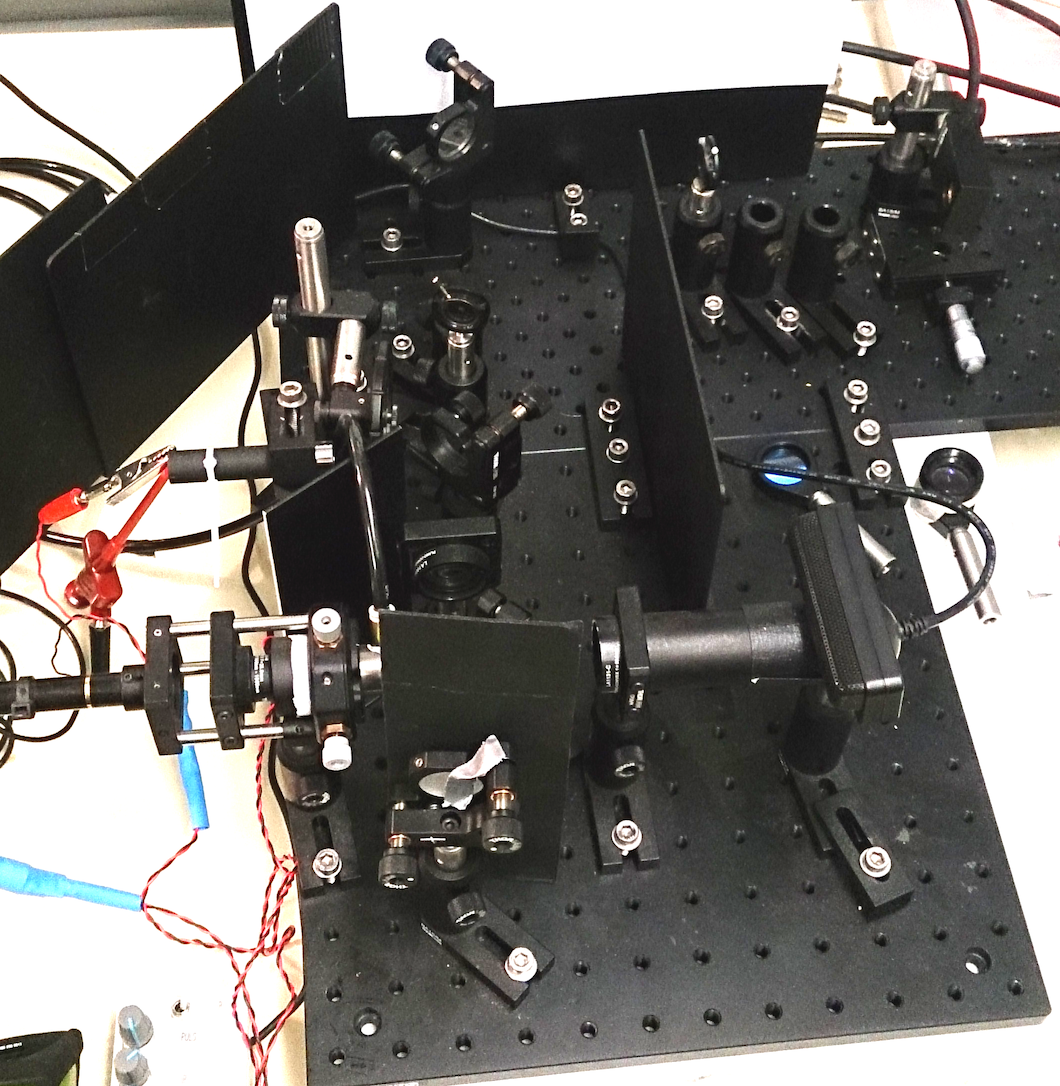
\includegraphics[scale=0.4]{../figures/aufbau.png}
	\caption{Setup with}
	\label{fig:setup}
\end{figure} 

\subsection{Catilever}
A cantilever is a tiny rod of about 1 to 3 mm long with a high reflective (> 99\%) mirror on top.
High reflectivity is needed because the highest force transfer and therefore pressure is obtained when all photons are reflected. We have a set of multiple cantilevers on a single plate \ref{fig:cantilever}.
\begin{figure}[H]
	\centering
	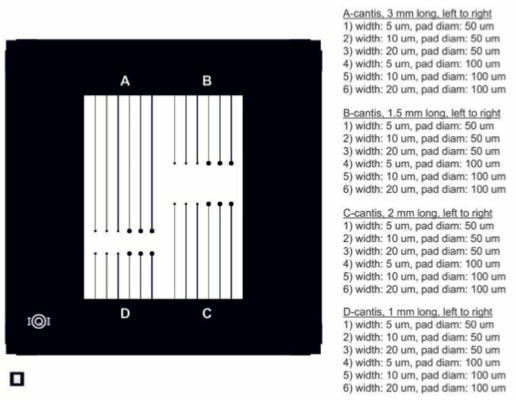
\includegraphics[scale=2]{../figures/cantilever.png}
	\caption{Multiple cantilever on one chip \cite{physikwiki}[p. 6]}
	\label{fig:cantilever}
\end{figure}





\pagebreak

\section{Measurement}
\subsection{Dampend driven harmonic oscilliation}
With a pulsed laser and a previous described cantilever we can build a oscillator that responds to the force of the photons. Because we want to measure a very tiny pressure the cantilever has to be driven by the pulsed laser at the resonance frequency of the oscillator. Due to the fact that we don't cool or evacuate our setup we have a non zero dampening.\\

\textbf{How to interpret the measurement}\\
Now combine the theory from \ref{theory} into one formula with the knowledge about the oscillator in \cite{physikwiki}[p. 3-5]:
$$\gamma = \frac{D}{m} = \frac{\omega_0}{Q}$$
From the equation of the harmonic driven dampened oscillator in \cite{physikwiki}[p. 3] we derive a formula for the position by using the ansatz $x(t) = x_0 e^{\omega t}$ in the equation with driving force:

$$x_0 = \frac{F_0}{m}  \frac{1}{\sqrt{ (\omega_0^2 - \omega^2 )^2 + \gamma^2  \omega^2}}$$
Because the interesting point is where $\omega_0 = \omega$ (resonance) we can set $\omega_0^2 - \omega^2$ to zero and get
$$x_0 = \frac{F_0}{m} * \frac{1}{\gamma  \omega}$$
using the definition for $\gamma$ and $\omega_0^2$ we get
$$k = \frac{F_0 * Q}{x_0}$$
for the spring constant k dependent on the force $F_0$ the quality factor Q and the displacement $x_0$. All these values can be measured and therefore we found a useful mathematical description of our system.\\
The $x_0$ is what we measure depending on the intensity of the laser, the displacement on the sensor (figure \ref{fig:sensorsensitivity}), the distance of the beam from cantilever to sensor and the length of the cantilever itself (resulting in a conversion factor from sensor result to displacement).\\

\subsection{Interferometer}
The interferometer is aligned that with no (or tiny) motion of the cantilever it is possible to see interference of the two rays on the wall. When the cantilever oscillates there is a phase shift which leads to a blurry pattern due to the rapid change of the pattern which the human eye cannot follow. This can be seen in figure \ref{fig:pattern}.

\begin{figure}[H]
	\centering
	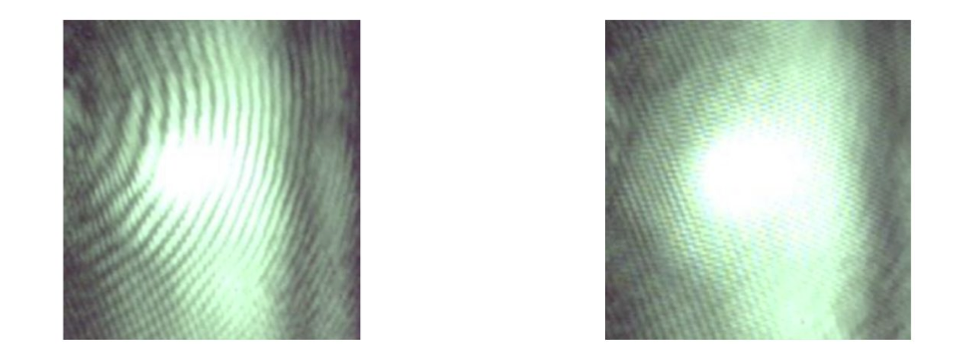
\includegraphics[scale=1]{../figures/interference.png}
	\caption{Left: Interference pattern without driving. Right: Interference with driving \cite{physikwiki}[p. 9, figure 5]}
	\label{fig:pattern}
\end{figure}

With this tool we can visually see on the wall 1m away if we found the resonance frequency. This can be very tricky because the eyes adjust to the color and pattern. Because there is a range of 3.5 kHz which may be stepped through in 10Hz steps we changed the observer of the pattern every 5 to 10 minutes. 



\subsection{Further steps}
\textbf{Classify some cantilever}\\
So now we have a chip (figure \ref{fig:cantilever}) with different cantilever on it.
A green laser built into a interferometer is used to observe the motion of the cantilever. \\
Using the PS3 camera we can adjust the speaker (and later the red laser) on the mirror of a single cantilever.
We now drive some of the cantilever with a acoustic speaker to find the resonance frequency of them.
Search for the resonance frequency was sweeping from 500Hz to 3.5kHz in steps of size 10Hz. This can be controlled with the oscilloscope.
The resonance frequency can be found by observing the pattern resulting from the interferometer on the wall which can be seen in figure \ref{fig:pattern}.
The results of this measurement are stated in table \ref{tab:acoustic_resonance}.\\
\\
\textbf{Detailed classification}\\
We now choose a cantilever for further experiments. In our case it is the 6D in figure \ref{fig:cantilever}.
To characterize the oscillator we sweep through the full frequency range of 10Hz-3.5kHz to get a resonance curve of our acoustic driven cantilever (figure \ref{fig:resonanzkurve}).\\
The result is fitted with a Lorentz curve. The full-width half maximum distance of the resonance curve represents the $\gamma$ factor of the oscillator. With the resonance frequency and the $\gamma$ factor the quality factor can be calculated .\\
\\
\textbf{Laser driven measurment}\\
After focusing both lasers with the PS3 cam on the cantilever and triggering the pulsed laser on the resonance frequency of the cantilever we can measure the displacement on the sensor. \\
Problem is that we don't yet know how to convert the signal from the sensor to a displacement of the cantilever.
We first measure the power of the red laser to determine the force. \\
After that we place the sensor on a moveable stage. By moving the sensor and taking note of the voltage and the distance on the nanometer screw we can determine a linear curve with a conversion factor represented as slope.
The fit can be seen in figure \ref{fig:sensorsensitivity} and the value of this constant C can be found in the results section (see \ref{label:values}).\\ 
Because the conversion is also dependent on the length of the interferometer we measure the length with a measuring tape (L in \ref{label:values}). The intensity (peak to peak on sine of interferometer) was also measured. Because the green laser changes it's intensity over the time of a measurement row we decided to normalize the values (figure \ref{fig:resonanzkurvedata} "LaserCountSum") and therefor also the transformation constant. The last part of calculating the conversion factor is the length of the cantilever itself which is 1mm.\\
So we calculate the proportional constant C in V/m (normalized 1/m see section \ref{label:results}) to get a displacement in meter on the sensor corresponding to the displacement of the cantilever.\\



\subsection{Final results}
With the values of the last section we are able to calculate the spring constant and the displacement of the cantilever. The results can be seen in section \ref{label:values}.\\
We have done some measurements around the resonance frequency to validate the peak.

%%%%%%%%%%%%%%%%%%%%%%%%%%%%%%%%%%%%%%%%%%%%%%%%
%%%%%%%%%%%%%%%%%%%%%%%%%%%%%%%%%%%%%%%%%%%%%%%%

\pagebreak

\section{Results}
\label{label:results}
The full document and the results contained in a QTI file and a Excel sheet can be found under \cite{github}.

\subsection{Acoustic measurment}

\begin{figure}[H]
 \centering
 \pgfplotstabletypeset[
 columns={cantilever, omega},
 col sep=&,
 columns/cantilever/.style={string type, column name=\makecell{$Name$\\ from \ref{fig:cantilever}} },
 columns/omega/.style={column name=\makecell{$f_{res}$ \\ ($\pm$ 10)[Hz]}, precision=0},
 every head row/.style={before row=\hline,after row=\hline\hline},
 every last row/.style={after row=\hline},
 every first column/.style={column type/.add={|}{} },
 every last column/.style={column type/.add={}{|} }
 ]{
 cantilever & omega
 A6 & 680
 D4 & 1870 
 D5 & 2565 
 D6 & 3395
 }
 \caption{Resonance frequency of four cantilever (acoustic driven)}
 \label{tab:acoustic_resonance}
\end{figure}

\subsection{Measurments on cantilever D4 graphics}

\begin{figure}[H]
	\centering
	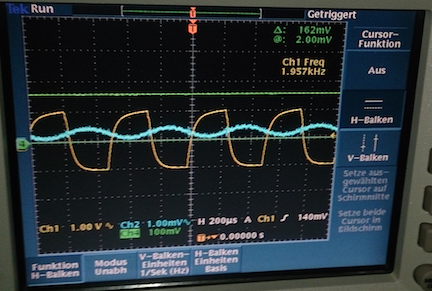
\includegraphics[scale=1]{../figures/messung.png}
	\caption{Measurement of data. Yellow:  Trigger for pulsed laser or acoustic drive. Cyan: Response on the sensor. Green: Interferometer power.}
	\label{fig:measurement}
\end{figure}

\begin{figure}[H]
	\centering
	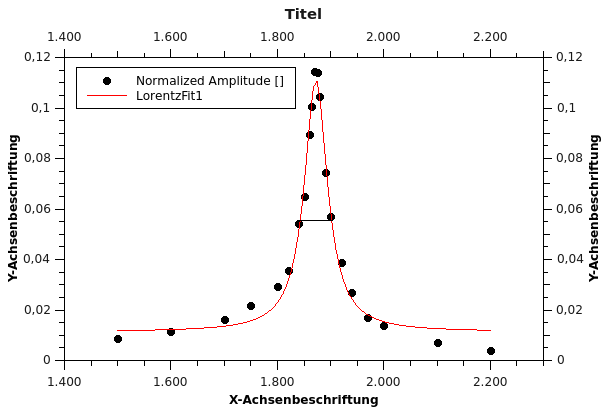
\includegraphics[scale=0.8]{../figures/Resonanzkurve.png}
	\caption{Resonance curve with Lorentz fit of acoustic driven cantilever D4}
	\label{fig:resonanzkurve}
\end{figure}

\begin{figure}[H]
	\centering
	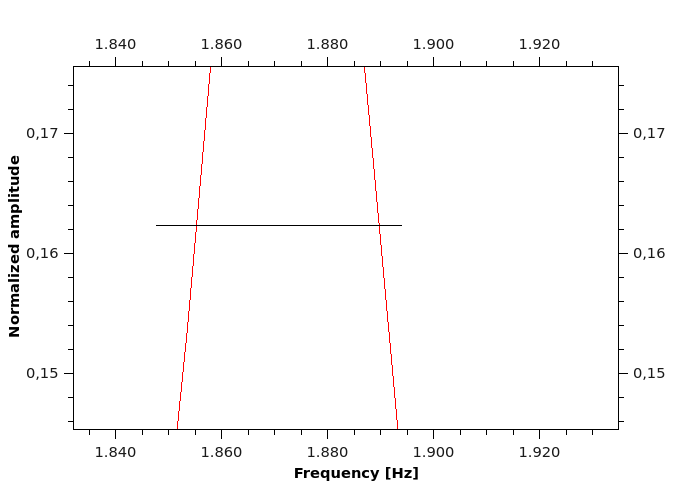
\includegraphics[scale=0.8]{../figures/ResonanzkurveHalbwertsbreite.png}
	\caption{Full width half maximum of the resonance curve of acoustic driven cantilever D4}
	\label{fig:resonanzkurvehmfuw}
\end{figure}


\begin{figure}[H]
	\centering
	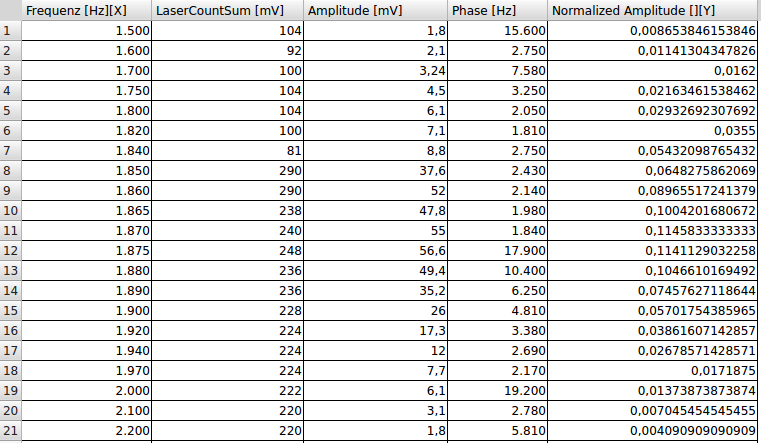
\includegraphics[scale=0.6]{../figures/rohdaten.png}
	\caption{Raw data determining the resonance curve of acoustic driven cantilever D4}
	\label{fig:resonanzkurvedata}
\end{figure}


\begin{figure}[H]
	\centering
	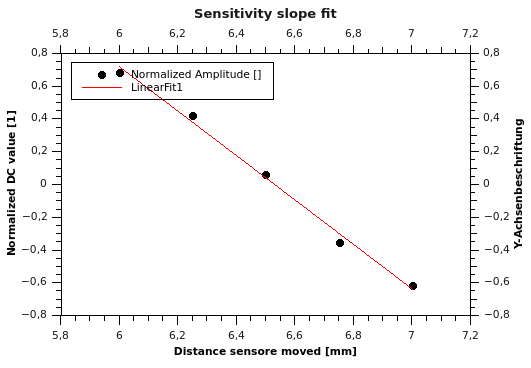
\includegraphics[scale=2]{../figures/Slopeofsensitivityofthesensor.png}
	\caption{Slope of the sensitivity of the quadrant sensor used to obtain the proportion constant C}
	\label{fig:sensorsensitivity}
\end{figure}

\noindent
\subsection{Values of measurments on cantilever D4}
\label{label:values}
Power of the red laser:
$$P = 1.45mW$$
The peak to peak Voltage of the green laser:
$$V_{PP} = (3.0 \pm 0.04)mV$$ 
Just for normalizing the result the intensity of the green laser:
$$I_{green} = (176 \pm 2.0) mV$$
The resonance frequency:
$$\omega_m = (11750 \pm 20) Hz$$
The length of the beam from the cantilever to the sensor:
$$L = (57.6 \pm 2)cm$$
Conversion factor for displacement on photodiode to oscillator displacement:
$$C = (1354 \pm 1) \frac{1}{m}$$ 
The FWHM $\gamma$ factor (graphic read out \ref{fig:resonanzkurvehmfuw}):
$$\gamma_m = (220 \pm 6) Hz$$
Quality factor of oscillator D4:
$$Q = (53 \pm 1)$$
Spring constant:
$$k = (47 \pm 1) \frac{mN}{m}$$
Displacement on resonance frequency:
$$x = (10.9 \pm 0.5) nm$$

%%%%%%%%%%%%%%%%%%%%%%%%%%%%%%%%%%%%%%%%%%%%%%%%
%%%%%%%%%%%%%%%%%%%%%%%%%%%%%%%%%%%%%%%%%%%%%%%%
\section{Discussion}
For a experiment at room temperature with normal air pressure and costs below \EUR{1000} one can learn and see a lot. \\
\\
The alignment process was done fast because the setup of the interferometer was already done. Getting the green and red laser on the cantilever was intuitive using the image of the PS3 camera. \\
\\
The acoustic driven measurements where annoying because the frequency for the 1mm cantilever had to be in the area of 1-3.5kHz which is a awful noise.\\
\\
The result of some nanometer displacement is in the area of what we were expecting of a 1mm cantilever. Problematic was the right use of the green laser because of the high fluctuations between measurements.\\
\\
Problematic till the end was how to calculate the correct displacement. The estimated value of the displacement is 5nm and therefore half of what we achieved and calculated. We thought we lost some 2$\pi$ on the way but the quality factor cancels out the 2$\pi$ of $\gamma_m$ and $\omega_m$ anyway. Maybe the transformation of the trigger signal to the used sinus would contribute a factor of 1/2.\\
\\
Due to the fact that some of our measurements were not very detailed in terms of accuracy (measure tape, jumping intensity) we took always a bigger error as calculated.\\


%%%%%%%%%%%%%%%%%%%%%%%%%%%%%%%%%%%%%%%%%%%%%%%%
%%%%%%%%%%%%%%%%%%%%%%%%%%%%%%%%%%%%%%%%%%%%%%%%

\bibliography{protocol.bib}
\bibliographystyle{plain}

%%%%%%%%%%%%%%%%%%%%%%%%%%%%%%%%%%%%%%%%%%%%%%%%
%%%%%%%%%%%%%%%%%%%%%%%%%%%%%%%%%%%%%%%%%%%%%%%%
							%BIS HIER VERBESSERT%
%%%%%%%%%%%%%%%%%%%%%%%%%%%%%%%%%%%%%%%%%%%%%%%%
%%%%%%%%%%%%%%%%%%%%%%%%%%%%%%%%%%%%%%%%%%%%%%%%

\end{document}